% !TEX root = paper.tex

\section{Evaluation}
\label{sec:eval}
\subsection{Experimental Settings}
\subsubsection{Datasets}

We collected the blood glucose dataset from July 2016 to January 2017. A total of 112 users joined in our experiments. During the experiments, each user wears a CGM device to collect the blood glucose sample every 3 minutes. Meanwhile, \sysname is installed in smartphones to sense the external factors.  Table.~\ref{dateset} details the experimental dataset. As is shown, the data of blood level shows the number of users in the four levels. The testing days date shows the user number at different testing days. The data of health status illustrates the health status of participants. The age, weight and gender shows the corresponding basic information of volunteers.

\subsubsection{Ground Truth and Metrics}

The blood glucose samples collected by the CGM are regarded as groundtruth. We compare the prediction results of \sysname with the groundtruth, and the performance is measured in terms of the precision \cite{}, recall\cite{} and accuracy\cite{}.

\begin{table}[]
\small
\centering
\caption{Details of the datasets
}
\label{dateset}
\begin{tabular}{|l|c|c|c|c|c|l|}
\hline
\textbf{Blood Level}                  & \textbf{Level 1}        & \textbf{Level 2}                      & \textbf{level 3}                       & \textbf{Level 4}                       & \multicolumn{2}{c|}{\textbf{Total}}             \\ \hline
\multicolumn{1}{|c|}{Number}          & 75369                   & 293530                                & 235686                                 & 158054                                 & \multicolumn{2}{c|}{762639}                     \\ \hline
\textbf{Testing days}                 & \textbf{5 $\sim$ 10 days}   & \textbf{10 $\sim$15 days}            & \textbf{15 $\sim$20 days}             & \textbf{20 $\sim$25 days}             & \multicolumn{2}{c|}{\textbf{25 $\sim$30 days}} \\ \hline
User number                           & 48                      & 24                                    & 20                                     & 13                                     & \multicolumn{2}{c|}{7}                          \\ \hline
\textbf{Health Status}                & \multicolumn{2}{c|}{\textbf{Health}}                            & \multicolumn{2}{c|}{\textbf{Type I}}                                            & \multicolumn{2}{c|}{\textbf{Type II}}           \\ \hline
User number                           & \multicolumn{2}{c|}{35}                                         & \multicolumn{2}{c|}{38}                                                         & \multicolumn{2}{c|}{39}                         \\ \hline
\multicolumn{1}{|c|}{\textbf{Age}}    & \textbf{15 $\sim$25}       & \textbf{25 $\sim$35}                     & \multicolumn{1}{l|}{\textbf{35 $\sim$45}} & \multicolumn{1}{l|}{\textbf{45 $\sim$55}} & \multicolumn{2}{l|}{\textbf{55 $\sim$70}}          \\ \hline
\multicolumn{1}{|c|}{User number}     & 8                       & 17                                    & 24                                     & 29                                     & \multicolumn{2}{c|}{34}                         \\ \hline
\textbf{Weight}                       & \textbf{30$\sim$45}        & \multicolumn{1}{l|}{\textbf{45$\sim$55}} & \multicolumn{1}{l|}{\textbf{55$\sim$65}}  & \multicolumn{1}{l|}{\textbf{65$\sim$75}}  & \multicolumn{2}{l|}{\textbf{75$\sim$90}}           \\ \hline
\multicolumn{1}{|c|}{User number}     & \multicolumn{1}{l|}{18} & \multicolumn{1}{l|}{21}               & \multicolumn{1}{l|}{32}                & \multicolumn{1}{l|}{22}                & \multicolumn{2}{l|}{19}                         \\ \hline
\multicolumn{1}{|c|}{\textbf{Gender}} & \multicolumn{2}{c|}{\textbf{Male}}                              & \multicolumn{4}{c|}{\textbf{Female}}                                                                                              \\ \hline
\multicolumn{1}{|c|}{User number}     & \multicolumn{2}{c|}{57}                                         & \multicolumn{4}{c|}{55}                                                                                                           \\ \hline
\end{tabular}
\end{table}

%
%
%\begin{table}[]
%\centering
%\caption{The details of dataset}
%\label{The details of dataset}
%\begin{tabular}{|l|c|c|c|c|l|}
%\hline
%\textbf{Blood Level}                  & \textbf{Level 1} & \textbf{Level 2} & \textbf{level 3} & \textbf{Level 4} & \textbf{Total}         \\ \hline
%\multicolumn{1}{|c|}{\textbf{Number}} & 75369            & 293530           & 235686           & 158054           & \multicolumn{1}{c|}{762639} \\ \hline
%\end{tabular}
%\end{table}















\begin{table}[]
\centering
\caption{Confusion matrix of \sysname performance}
\label{tab:confusion_matrix}
\begin{tabular}{|c|c|c|c|c|l|l|}
\hline
\multirow{2}{*}{\textbf{\begin{tabular}[c]{@{}c@{}}Ground\\ Truth\end{tabular}}} & \multicolumn{4}{c|}{\textbf{Predictions}}                                                                                 & \multicolumn{2}{l|}{\multirow{2}{*}{}}                                                            \\ \cline{2-5}
                                                                                 & Level 1                      & Level 2                      & Level 3                      & Level 4                      & \multicolumn{2}{l|}{}                                                                             \\ \hline
Level 1                                                                          & \cellcolor[gray]{0.8}62657                        & 5521                         & 3672                         & 3519                         & 83.13\%                             & \multirow{4}{*}{\rotatebox{90}{\textbf{Recall}} }                           \\ \cline{1-6}
Level 2                                                                          & 16346                        &  \cellcolor[gray]{0.8}240584                       & 27563                        & 9037                         & 81.96\%                             &                                                             \\ \cline{1-6}
Level 3                                                                          & 2660                         & 30905                        & \cellcolor[gray]{0.8}188472                       & 13649                        & 79.97\%                             &                                                             \\ \cline{1-6}
Level 4                                                                          & 3443                         & 5620                         & 14278                        & \cellcolor[gray]{0.8}134713                       & 85.23\%                             &                                                             \\ \hline
\multicolumn{1}{|l|}{\multirow{2}{*}{}}                                          & \multicolumn{1}{l|}{73.62\%} & \multicolumn{1}{l|}{85.12\%} & \multicolumn{1}{l|}{80.55\%} & \multicolumn{1}{l|}{83.72\%} & \multicolumn{2}{l|}{\multirow{2}{*}{\begin{tabular}[c]{@{}l@{}}Accuracy:\\ 82.14\%\end{tabular}}} \\ \cline{2-5}
\multicolumn{1}{|l|}{}                                                           & \multicolumn{4}{c|}{\textbf{Precision}}                                                                                 & \multicolumn{2}{l|}{}                                                                             \\ \hline
\end{tabular}
\end{table}



\subsubsection{System Evaluation}

To evaluate the \sysname performance, we provide CGM for each new user for one time usage, supporting more than 5 days. We take the former 4 days as the training data, and left days as the testing data. If the left days of one users are longer than 2 days, we calculate the user's average performance. Table~\ref{tab:confusion_matrix} shows the results of testing dataset. As we can see,  the recalls of four blood glucose levels are above 79\%, and all the precisions of four blood glucose levels keep above 73\%. In particular, the recalls of level 1 and level 3 are 83.13\% and 85.23\%, demonstrating the high sensitivity of \sysname towards these two levels. The 82.14\% accuracy states the outstanding prediction performance of \sysname.



\begin{figure}[!t]
\centering
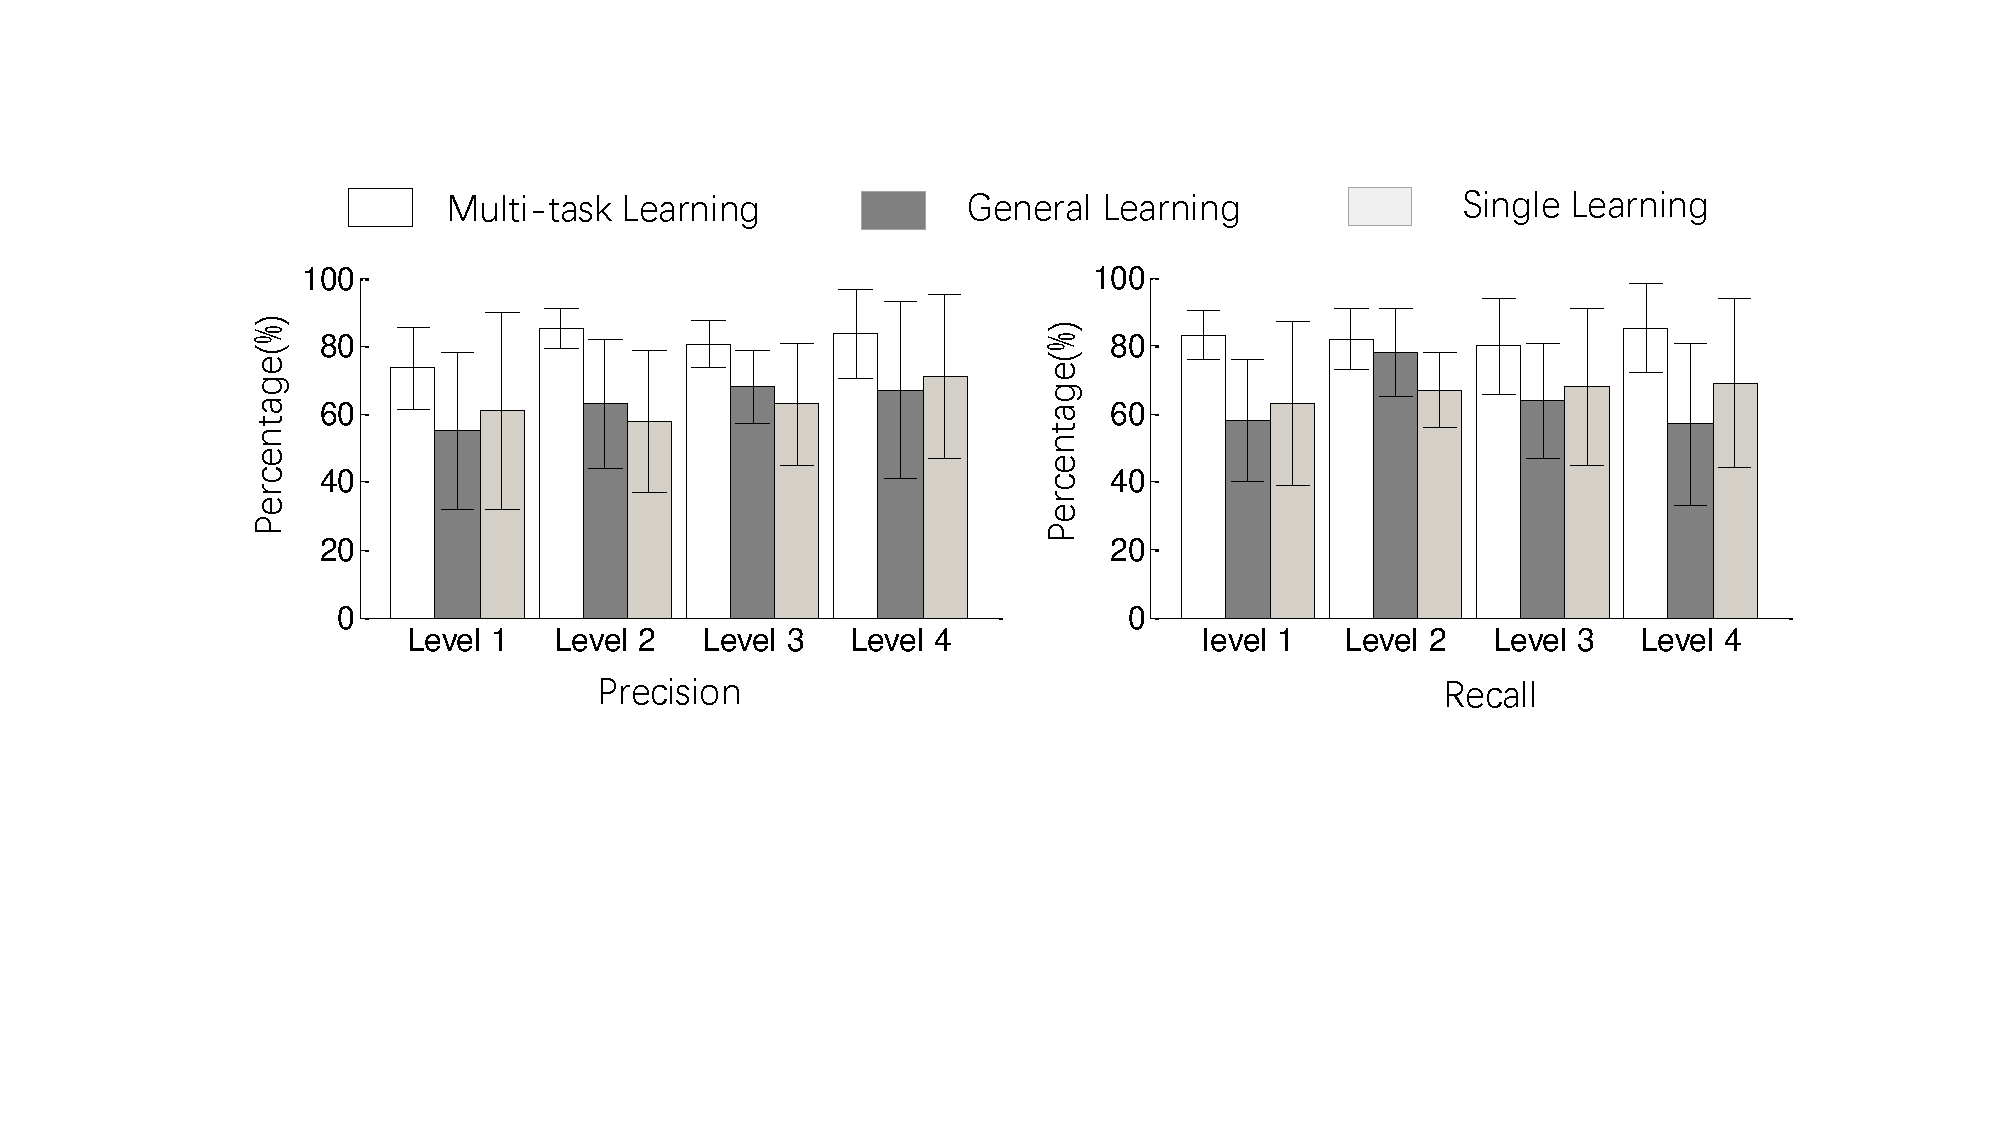
\includegraphics[width=0.9\columnwidth]{./img/CMP_Models.pdf}
\caption{The model comparison}
\label{fig:cmp_model}
\end{figure}

\paragraph{Evaluation with various training data}

Since the users may wear CGM continuously, we evaluate the performance of \sysname with increasement of training dataset by five days. Under each system evaluation, we trained all the data of the users with before the testing date, and measured the system by calculating the average performance of those who have longer testing days.

Fig.~\ref{fig:per_under_train_days} illustrates the results. We can see the system performance grow up with the increasement of training dataset, demonstrating the performance of \sysname will grow up with more training data.


\begin{figure}[!t]
\centering
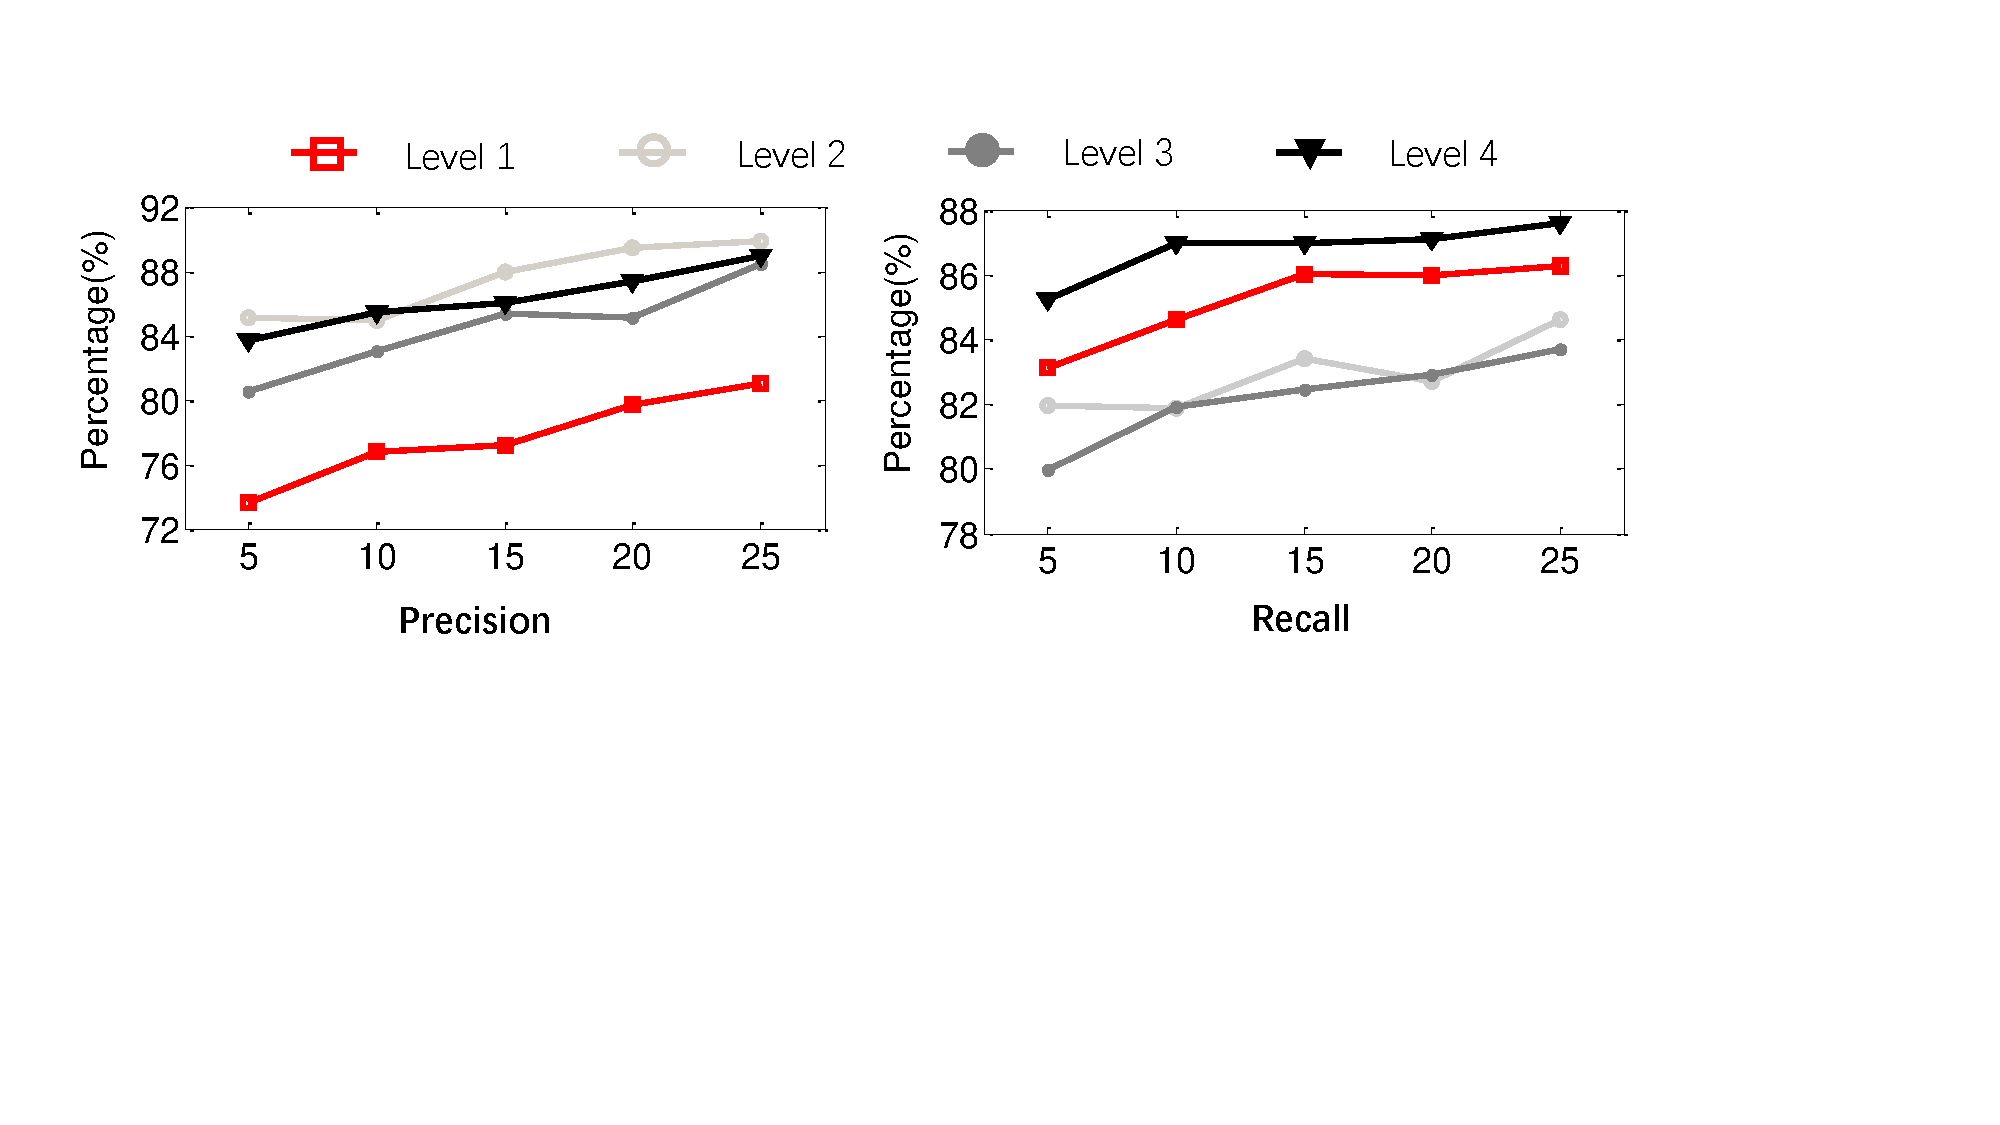
\includegraphics[width=0.9\columnwidth]{./img/performance_under_days.pdf}
\caption{System performance under different training date}
\label{fig:per_under_train_days}
\end{figure}



\paragraph{Evaluation with various prediction duration}

Considering the uncertainties of blood glucose increase while the time passing by, we detail the system performance by differentiating the prediction durations in  Fig.~\ref{fig:per_under_various_pred_days}.
As expected, the system performance shows a decrease trend while the prediction duration leave longer away. It is possible due to the internal relevant factors of blood glucose changed with the time passing by. However, the system performance still can maintain an acceptable level for 30-days prediction.



\begin{figure}[!t]
\centering
\includegraphics[width=0.9\columnwidth]{./img/Performance under prediction
longer.pdf}
\caption{System performance under different prediction duration}
\label{fig:per_under_various_pred_days}
\end{figure}



\subsubsection{Evaluation on Multi-task Model structure}
To demonstrate the effectiveness of \modelname structure, we compared our model over the following combinations.

\begin{itemize}

  \item \emph{General Learning}:
  All the users shared a same information representation, dynamic and personality layers, which assumes the blood glucose trends of all users can be tracked by a same model.


  \item \emph{Single Learning }:
  Each user is trained for a specific model.

  Fig.~\ref{fig:cmp_model} shows the results.
\end{itemize}

\subsubsection{Evaluation on Features}

We show the effectiveness of four-dimensional feature in Table ~\ref{Feature_Evaluation}. Clearly, the tracking performance of \sysname improve a lot by adding one feature set into the model.



\begin{table}[]
\small
\centering
\caption{Feature Evaluation}
\label{Feature_Evaluation}
\begin{tabular}{|c|c|c|c|c|c|c|c|c|}
\hline
                                   & \multicolumn{2}{c|}{\textbf{Level 1}}                     & \multicolumn{2}{c|}{\textbf{Level 2}} & \multicolumn{2}{c|}{\textbf{Level 3}}                     & \multicolumn{2}{c|}{\textbf{Level 4}}                     \\ \hline
\textbf{Features}                  & \textbf{Precision} & \multicolumn{1}{l|}{\textbf{Recall}} & \textbf{Precision}  & \textbf{Recall} & \textbf{Precision} & \multicolumn{1}{l|}{\textbf{Recall}} & \textbf{Precision} & \multicolumn{1}{l|}{\textbf{Recall}} \\ \hline
$F_{p}$                            & 43.37$\%$               & 32.82$\%$                                 & 46.03$\%$                & 39.10$\%$            & 51.79$\%$               & 48.95$\%$                                 & 56.30$\%$               & 43.49$\%$                                 \\ \hline
$F_{p}$+$F_{t1}$                   & 51.97$\%$               & 58.11$\%$                                 & 60.42$\%$                & 58.90$\%$            & 63.35$\%$               & 53.59$\%$                                 & 69.82$\%$               & 55.16$\%$                                 \\ \hline
$F_{p}$+$F_{t1}$+$F_{t2}$          & 64.60$\%$               & 73.08$\%$                                 & 69.87$\%$                & 61.23$\%$            & 74.33$\%$               & 67.81$\%$                                 & 76.64$\%$               & 72.32$\%$                                 \\ \hline
$F_{p}$+$F_{t1}$+$F_{t2}$+$F_{t3}$ & 73.62$\%$   & 83.13$\%$                                 & 83.13$\%$               & 83.13$\%$            & 80.55$\%$   & 79.97$\%$
& 83.72$\%$               & 85.23$\%$                                  \\ \hline
\end{tabular}
\end{table}


\subsubsection{Blood glucose level predictions}

Fig.~\ref{fig:pre_gt} compares the predictive results of \sysname and true blood glucose level of a user over one day.




\begin{figure}[!t]
\centering
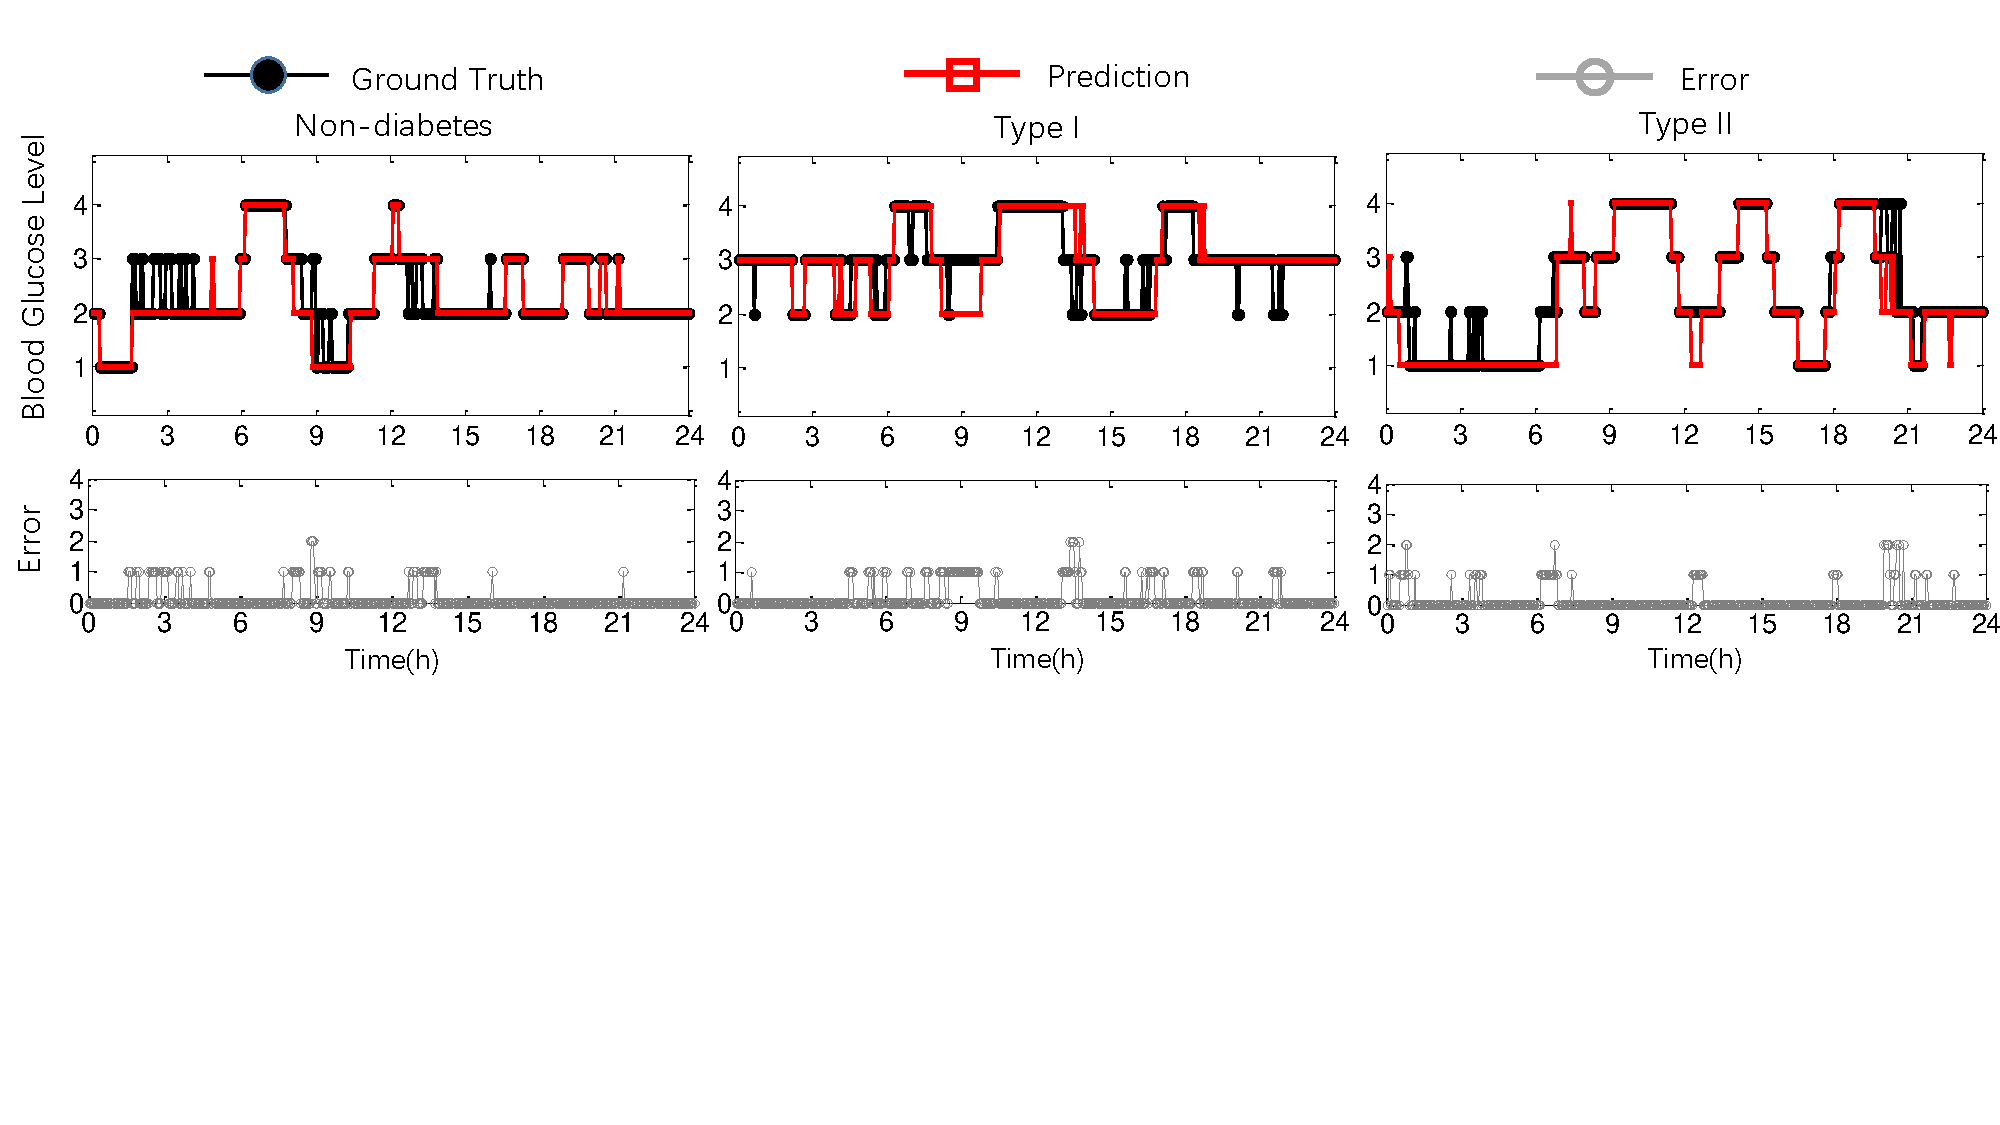
\includegraphics[width=0.5\columnwidth]{./img/pred_vs_gt.pdf}
\caption{The comparison of prediction and the ground truths of one user.}
\label{fig:pre_gt}
\end{figure}


\subsubsection{Model comparison}

We compare \modelname of \sysname over following baselines:

1) Gradient Boosting (GB):

2) Support Vehicle Machine (SVM):

3) Hidden Markov model (HMM):

4) Linear Regression (LR):

5) Random Forest (RF):

6) Gaussian Processes (GP):





